\documentclass[10pt,xcolor={dvipsnames}]{beamer}
\usetheme[progressbar=frametitle]{PaloAlto}
\usepackage{appendixnumberbeamer}
\usepackage{booktabs}
\usepackage[scale=2]{ccicons}
\usepackage{pgfplots}
\usepgfplotslibrary{dateplot}
\usepackage[utf8]{inputenc}
\usepackage{fancyvrb}
\usepackage{xspace}
\newcommand\tab[1][1cm]{\hspace*{#1}}
\usepackage{pgf-pie}


\begin{document}

     
    \subsection{Gráfico Barras}
        \begin{frame}[fragile]{Histograma} 
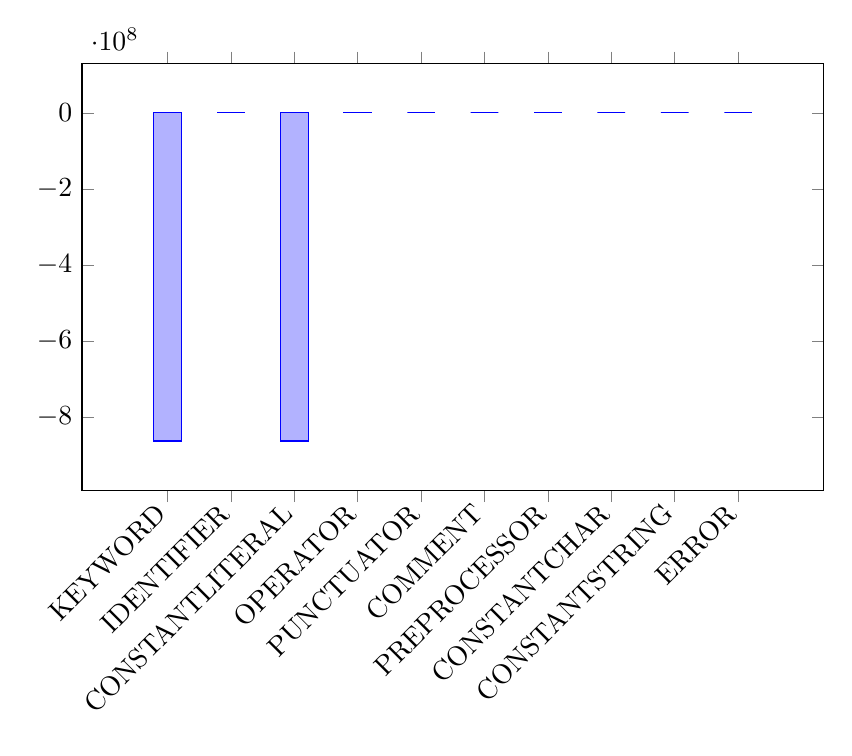
\begin{tikzpicture}     
\begin{axis}[ybar, enlargelimits=0.15, x tick label style={rotate=45, anchor=east},    symbolic x coords={KEYWORD, 
IDENTIFIER, 
CONSTANTLITERAL, 
OPERATOR, 
PUNCTUATOR, 
COMMENT, 
PREPROCESSOR, 
CONSTANTCHAR, 
CONSTANTSTRING, 
ERROR, 
},xtick=data,width=11cm,height=7cm] 
 \addplot coordinates {(KEYWORD,-863060829) 
(IDENTIFIER,32722) 
(CONSTANTLITERAL,-863060830) 
(OPERATOR,32716) 
(PUNCTUATOR,15) 
(COMMENT,0) 
(PREPROCESSOR,0) 
(CONSTANTCHAR,0) 
(CONSTANTSTRING,0) 
(ERROR,0) 
};
\end{axis}  
\end{tikzpicture} 
\end{frame}    
    \subsection{Gráfico Pastel}
        \begin{frame}[fragile]{Histograma} 
\begin{tikzpicture} 
\pie[text=legend]{ 7/KEYWORD, 18/IDENTIFIER, 7/CONSTANTLITERAL, 7/OPERATOR, 47/PUNCTUATOR, 5/COMMENT, 0/PREPROCESSOR, 0/CONSTANTCHAR, 7/CONSTANTSTRING, 0/ERROR, }
\end{tikzpicture}
\end{frame}
    
    
    \section{Analisis Léxico}

        \begin{frame}[fragile,allowframebreaks]{Resaltado de sintaxis}~\newline\newline\color{Sepia}\verb$int$ \color{BlueViolet}\verb$FUNCION$\color{OliveGreen}\verb$($\color{OliveGreen}\verb$)$ \color{OliveGreen}\verb${$\newline \color{Sepia}\verb$int$ \color{BlueViolet}\verb$a$ \color{OliveGreen}\verb$=$ \color{BurntOrange}\verb$3$\color{OliveGreen}\verb$;$\newline \color{Sepia}\verb$return$ \color{BlueViolet}\verb$a$\color{OliveGreen}\verb$;$\newline\color{OliveGreen}\verb$}$\newline\newline\newline\color{Sepia}\verb$int$ \color{BlueViolet}\verb$main$\color{OliveGreen}\verb$($\color{OliveGreen}\verb$)$\color{OliveGreen}\verb${$\newline    \newline    \color{BlueViolet}\verb$FUNCION$\color{OliveGreen}\verb$($\color{OliveGreen}\verb$)$\color{OliveGreen}\verb$;$\newline    \color{Sepia}\verb$int$ \color{BlueViolet}\verb$a$ \color{OliveGreen}\verb$=$ \color{BurntOrange}\verb$9$\color{OliveGreen}\verb$;$\newline    \color{BlueViolet}\verb$a$ \color{ProcessBlue}\verb$+$\color{OliveGreen}\verb$=$ \color{BurntOrange}\verb$7$\color{OliveGreen}\verb$;$\newline\newline\newline    \color{BlueViolet}\verb$printf$\color{OliveGreen}\verb$($\color{BlueViolet}\verb$a$\color{OliveGreen}\verb$)$\color{OliveGreen}\verb$;$\newline\color{OliveGreen}\verb$}$\newline
\end{frame}



\end{document}
